
L'obiettivo della tesi è implementare un'architettura Function as a Service (FaaS) in cui le funzioni siano compilate come moduli WebAssembly (Wasm). L'approccio adottato mira a semplificare il processo di sviluppo, evitando che l'utente debba definire esplicitamente le caratteristiche tecniche dei moduli Wasm, consentendo così un'esperienza di utilizzo più astratta e focalizzata sulla logica applicativa.\\
In questo capitolo verranno mostrati i possibili scenari di sviluppo e verrà descritta la soluzione scelta, andando ad analizzarne i benefici e le criticità. 

\section{Infrastruttura}

L'analisi dell'infrastruttura ha inizio con l'individuazione dei requisiti fondamentali su cui si basa la soluzione proposta. Tali requisiti definiscono le caratteristiche essenziali per garantire il corretto funzionamento e l'efficienza del sistema.\\
In primo luogo, l'architettura si fonda sul modello di Edge Computing[\ref{fig:modello_edge_computing}], che prevede l'elaborazione dei dati in prossimità della fonte di generazione, al fine di ridurre la latenza e migliorare le prestazioni complessive del sistema. È quindi necessario identificare le tecnologie da utilizzare per simulare nodi Cloud, Edge ed IoT.\\
Un ulteriore requisito è la presenza di un runtime WebAssembly su ciascun nodo dell'infrastruttura, necessario per l'esecuzione delle funzioni applicative in modo portabile e isolato. È inoltre imprescindibile garantire la comunicazione tra i diversi runtime distribuiti, così da consentire la cooperazione tra i nodi e l'instradamento delle richieste in maniera efficiente.
Questo requisito, dato che i moduli seguono il paradigma FaaS, richiede l'utilizzo di un sistema di messaggistica basato su eventi come quello \texttt{Pub/Sub}. \\
Infine, l'infrastruttura deve essere progettata per assicurare la scalabilità e la redistribuzione delle funzioni in caso di guasto, garantendo così l'affidabilità del sistema e la continuità operativa.

\FloatBarrier
\begin{figure}[h]
    \centering
    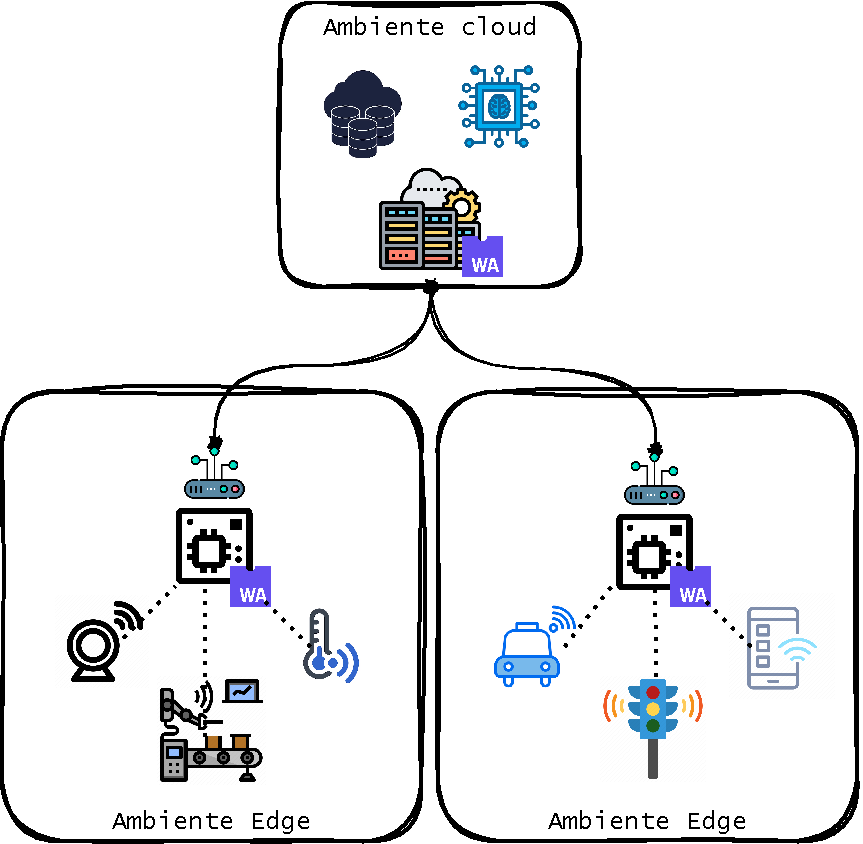
\includegraphics[width=0.8\textwidth]{img/schemi/schemi-Scenari.drawio.pdf}
    \caption{Modello Edge Computing}
    \label{fig:modello_edge_computing}
\end{figure}
\FloatBarrier

\subsection{Scelta del runtime WASM}

È quindi necessario utilizzare un framework o runtime WASM che soddisfi i seguenti requisiti:
\begin{itemize}
    \item Compatibilità sia con ambienti Cloud-Native (come Kubernetes, Docker) che tradizionali (bare-metal con Linux), in modo da non imporre dei requisiti forti nel deployment dell'infrastruttura
    \item Gestione dell'offloading fra nodi differenti, requisito fondamentale dato che uno degli scopi del progetto è predisporre una struttura FaaS che possa eseguire sia su nodi Cloud che Edge
    \item Facile configurazione e scalabilità dei runtime
    \item Supporto di una modalità di deployment dei moduli WASM automatizzabile e dichiarativa, così da facilitare l'implementazione del framework sviluppato per questo progetto
\end{itemize}

Verranno adesso elencati e descritti tutti gli approcci e i tool che sono stati esplorati prima di giungere alla soluzione adottata nel progetto.

\subsubsection{Runtime standalone}

L'approccio più semplice ed immediato è stato quello di utilizzare uno dei tanti runtime WebAssembly disponibili sul mercato per eseguire i moduli precompilati. In particolare il workflow consisteva nel:
\begin{enumerate}
    \item Sviluppare il programma in un linguaggio che supporta Wasm (in questo caso Golang)
    \item Utilizzare un compilatore per generare un modulo WebAssembly. Nel caso di Golang ci sono due opzioni disponibili:
    \begin{itemize}
        \item Default compiler di Golang -- \lstinline{GOOS=js GOARCH=wasm go build -o main.wasm}
        \item TinyGo -- \lstinline{GOOS=js GOARCH=wasm tinygo build -o main.wasm ./main.go}
    \end{itemize}
    
    \item Eseguire il modulo in un runtime Wasm. In questo caso è stato utilizzato Wasmtime:
    \lstinline{wasmtime serve -S main.wasm}
\end{enumerate}

Sebbene questo approccio sia il più leggero ed il più facile da implementare, manca dei requisiti chiave del nostro progetto:
\begin{itemize}
    \item Scalabilità automatica fra i nodi
    \item Approccio FaaS difficilmente applicabile data la mancanza di un deployment tramite file descrittivo (come succede in Kubernetes o Docker)
    \item Necessità di implementare tutta l'infrastruttura di networking e il routing fra i moduli Wasm
\end{itemize}

\subsubsection{Dockerfile e containerd}

Il passo successivo è stato approfondire l'integrazione fra i moduli Wasm e i container runtime tradizionali, resa possibile dall'implementazione della specifica OCI. Fra i CR che supportano moduli Wasm il più accessibile è la release beta di \texttt{containerd}\cite{containerd_runwasi}, installabile facilmente anche da client come Docker Desktop[\ref{fig:docker_desktop}].

\FloatBarrier
\begin{figure}[h]
    \centering
    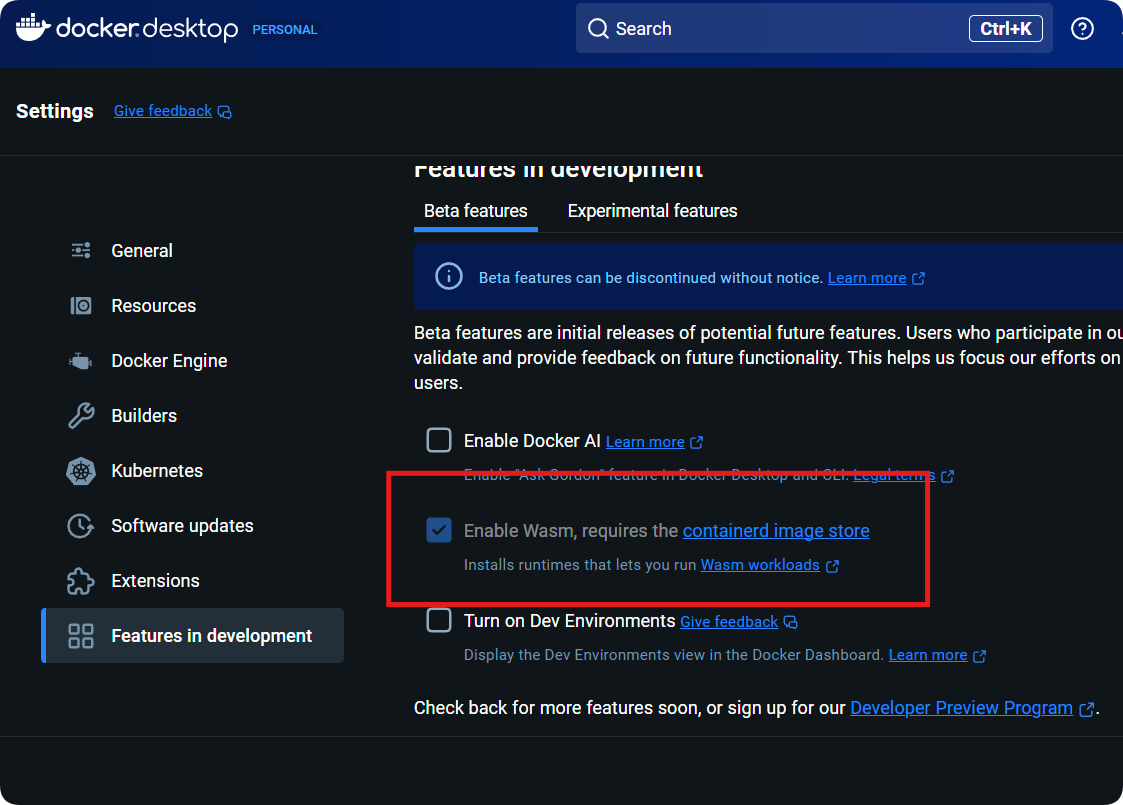
\includegraphics[width=0.7\textwidth]{img/wasm_docker_desktop.png}
    \caption{Opzione Wasm su Docker Desktop}
    \label{fig:docker_desktop}
\end{figure}
\FloatBarrier

Grazie a questa feature è possibile incorporare dei moduli Wasm all'interno di container utilizzando un semplice Dockerfile[\ref{code:dockerfile_example_wasm}] come il seguente:
\begin{lstlisting}[language=Dockerfile, caption={Esempio Dockerfile per modulo Wasm}, captionpos=b, label={code:dockerfile_example_wasm}]
    FROM scratch
    
    COPY ./main.wasm /main.wasm
    
    CMD ["serve","./main.wasm"]
\end{lstlisting}
Grazie alla gestione dei container possiamo risolvere problemi come la scalabilità e il networking sul singolo nodo: utilizzando strumenti come Docker Compose (già ampiamente descritto nella sezione \ref{sec:dockercompose} è possibile impostare il numero di repliche di un container (per risolvere la scalabilità) ed utilizzare il nome del servizio associato per il routing dei messaggi. Rimane però il problema dell'offloading fra nodi diversi: tecnologie come Docker Swarm e Kubernetes, fatte per gestire e bilanciare il carico computazionale fra più nodi di un cluster, necessitano ovviamente di essere installate in tutta l'infrastruttura target.\\
In questa situazione una soluzione come SpinKube, che sfrutta al massimo le potenzialità di Kubernetes per gestire moduli Wasm, potrebbe trovare una buona applicazione.\\
Purtroppo nel nostro caso non possiamo garantire che Cloud ed Edge abbiano a disposizione la stessa infrastruttura e necessitiamo di una soluzione che possa funzionare sia su ambienti Cloud-Native che in ambienti più tradizionali, come una semplice VM Linux.\\
Oltre ai problemi infrastrutturali della gestione multi-nodo rimane in sospeso la questione del routing e del discovery dei vari moduli: in un modello FaaS ogni task deve avere un'interfaccia definita e deve poter essere raggiunta indipendentemente dal nodo in cui essa sta essendo eseguita. Questa problematica, benché chiara dall'inizio del progetto, difficilmente è risolvibile tramite uno sviluppo puntuale che non faccia uso di tecnologie già affermate.

\subsubsection{wRPC}
\label{sec:wrpc}

Per risolvere i problemi legati al discovery ed alla chiamata di task remote ho tentato di implementare in ogni modulo wasm un server RPC (\texttt{Remote Procedure Call}). Il tenologia RPC è infatti molto adatta ad implementare il modello FaaS, dato che consente di esporre un'interfaccia stabile per poter eseguire delle procedure remote indipendentemente da dove questa stia girando.\\
In questa fase di ricerca mi sono imbattuto nel progetto \texttt{wRPC}\cite{bytecodealliance_wrpc}, un framework RPC della Bytecode Alliance (l'organizzazione che si occupa di sviluppare e mantenere le tecnologie legate a WebAssembly, come WASI\cite{WASI2024} e runwasi\cite{containerd_runwasi} di conteinerd).\\
wRPC è un protocollo indipendente dal trasporto, progettato per facilitare l'esecuzione di funzionalità definite in WIT (WebAssembly Interface Types) su reti o altri mezzi di comunicazione. Le sue principali applicazioni includono:
\begin{itemize}
    \item Plugin runtime WebAssembly esterni
    \item Comunicazione distribuita tra componenti WebAssembly
\end{itemize}
Sebbene wRPC sia stato progettato principalmente per i componenti Wasm, è completamente utilizzabile anche al di fuori del contesto WebAssembly, servendo come framework RPC generico. Utilizza la codifica della definizione del valore del modello dei componenti durante la trasmissione e supporta sia casi d'uso dinamici (basati, ad esempio, sull'introspezione del tipo di componente WebAssembly a runtime) che statici. Per i casi d'uso statici, wRPC fornisce generatori di binding WIT per Rust e Go.\\
Anche se questo framework semplifica notevolmente il processo di deployment dei componenti Wasm risulta difficile da configurare dinamicamente partendo da una semplice task, cioè lo scopo di questo progetto.



\section{Definizione del workflow}

Ora che l'infrastruttura in cui verranno eseguiti i task è chiara analizziamo quello che sarà il workflow, partendo dal definire la struttura del progetto, le modalità di definizione dei singoli moduli Wasm.

 \subsection{Struttura del progetto}
\label{sec:framework_structure}

Il framework sviluppato in questo elaborato deve soddisfare ai seguenti requisiti:
\begin{itemize}
    \item Fornire un modo intuitivo per istanziare un modulo FaaS, quindi ridurre al minimo le responsabilità dell'utilizzatore che dovrà esclusivamente specificare la il codice della funzione da eseguire nella task remota
    \item Astrarre i più possibile il processo di generazione del codice e di build del componente Wasm
    \item Consentire all'utilizzatore di configurare i metadati delle task, come il nome, il target di deployment ed origine e destinazione dei dati
\end{itemize}
È inoltre necessario configurare un sistema di comunicazione che consenta di trasferire i messaggi fra i componenti Wasm, indipendentemente da dove essi siano deployati. Per ottenere questo risultato le applicazioni si appoggiano ad una piattaforma di messaggistica con modello Pub/Sub.\\
Tenendo a mente ciò la soluzione è stata comporre un ``progetto'' contenente tutte le informazioni necessarie per gestire l'intera pipeline e strutturato nel seguente modo:\\

\texttt{project/}
\dirtree{%
.1 workflow.yaml.
.1 tasks/.
.2 sensor\_read.go.
.2 aggregate.go.
.1 gen/.
}

\vspace{0.5cm}

\subsection{Workflow manifest}

Analizziamo ora gli elementi che compongono il progetto, partendo dal file \texttt{workflow.yaml}.
All'interno di questo file, formattato in sintassi Yaml, viene descritta una lista di \textbf{task}: ogni task corrisponde ad un componente Wasm e i suoi provider eseguito su wasmCloud. Per ogni task è possibile specificare una serie di configurazioni:

\begin{lstlisting}[language=yaml, caption={Esempio workflow.yaml}, captionpos=b, label={code:workflow_example}]
    project_name: Test_project
    tasks:
      - name: Temp sensor read
        type: producer_nats
        code: sensor_read.go
        targets:
          - cloud
          - edge
        source_topic: test_source_data
        dest_topic: test_dest_data
        component_name: temp_sensor_data
        version: 1.0.0
    ...
\end{lstlisting}

Basandoci sul file di esempio[\ref{code:workflow_example}] analizziamo i vari campi specificati nella task:
\begin{itemize}
    \item \texttt{name} -- nome della task mostrato nei log e nelle descrizioni
    \item \texttt{type} -- template utilizzato per la generazione del codice, verranno dati ulteriori dettagli in seguito
    \item \texttt{code} -- nome del file (situato nella cartella \texttt{tasks/} contenente il codice da inserire nella task
    \item \texttt{targets} -- label dei nodi in cui verrà deployata l'applicazione
    \item \texttt{source\_topic} e \texttt{dest\_topic} -- topic utilizzati dall'applicazione per ottenere e consegnare i messaggi. La presenza di questi due campi può variare o meno in base al template selezionato
    \item \texttt{component\_name} e \texttt{version} -- conferiranno il nome al componente Wasm e all'artifact OCI corrispondente in fase di Build
\end{itemize}

All'interno della directory \texttt{task} vengono inseriti i file contenente il codice delle funzioni (che verrà poi utilizzato in fase di generazione), inoltre è presente la cartella \texttt{gen} dove verranno inseriti i progetti contenente il codice generato dal framework.

\section{Generazione del codice}

Una volta definito il progetto è possibile sfruttare il framework per generare il codice e i manifest necessari in seguito, il processo segue i seguenti step edè  schematizzato nella seguente figura \ref{fig:code_gen_pipeline}:

\begin{enumerate}
    \item creazione o pulizia della cartella \texttt{gen/}
    \item parsing del file \texttt{workflow.yaml}
    \item per ogni task presente sul file workflow:
    \begin{enumerate}
        \item creazione della cartella dedicata al componente sotto \texttt{gen/}. Il nome è preso dal campo \texttt{component\_name}
        
        \item selezione dei template da utilizzare come base del codice in base al campo \texttt{type} e copia dei files dentro la cartella dedicata
        
        \item ricerca e copia del file specificato nel campo \texttt{code}
        
        \item sostituzione dei valori nel template con quelli della task specificata nel file workflow
    \end{enumerate}
\end{enumerate}

\FloatBarrier
\begin{figure}[h]
    \centering
    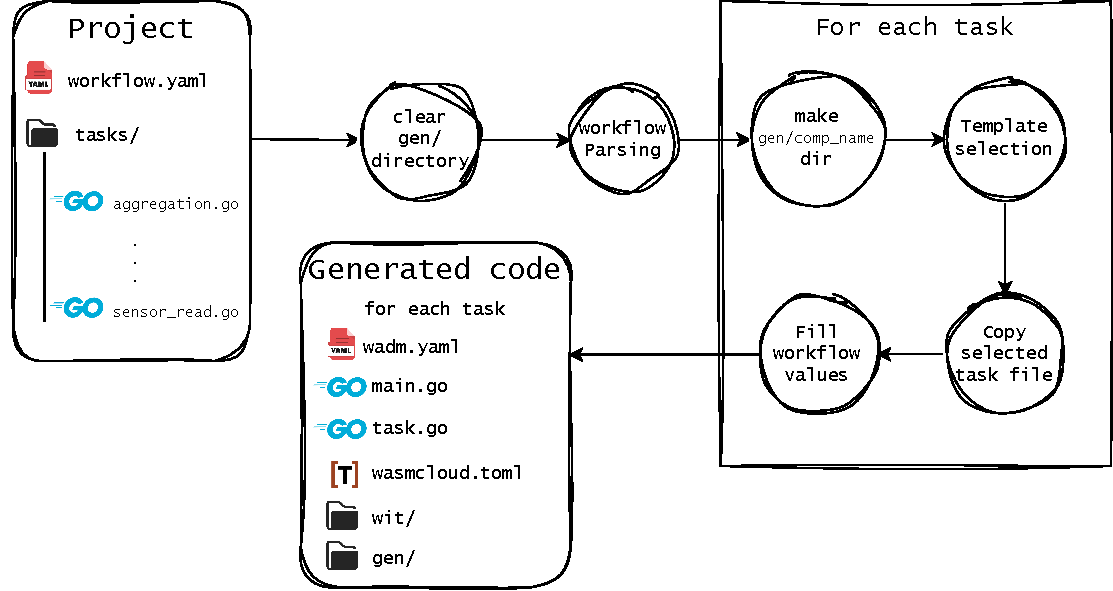
\includegraphics[width=0.8\textwidth]{img/schemi/schemi-architettura-generazione.drawio.pdf}
    \caption{Processo generazione codice}
    \label{fig:code_gen_pipeline}
\end{figure}
\FloatBarrier

\section{Build del Componente Wasm}

Una volta generato il codice nella cartella \texttt{gen} saranno presenti tante directory contenenti il codice generato necessario per buildare il componente Wasm e deployarlo su wasmCloud.\\
Il processo di build si suddivide in tre step principali (per ogni cartella presente dentro \texttt{gen}):
\begin{enumerate}
    \item istanziamento del container contenente i tool per buildare il codice \texttt{wash-build-image} e mount dinamico della cartella con il codice generato
    \item scaricamento dipendenze Golang (se necessario) e build del componente Wasm con la toolchain di wasmCloud (comando \texttt{wash build})
    \item push dell'OCI artifact (il componente Wasm buildato) sul registry remoto configurato
\end{enumerate}
Una versione schematica del processo è visibile dalla seguente immagine:

\FloatBarrier
\begin{figure}[h]
    \centering
    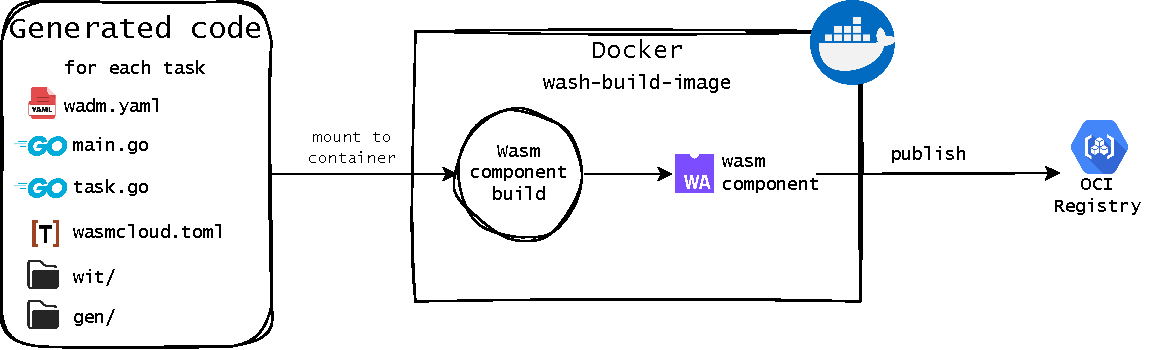
\includegraphics[width=0.8\textwidth]{img/schemi/schemi-architettura-build.drawio.pdf}
    \caption{Processo build componente Wasm}
    \label{fig:code_build_pipeline}
\end{figure}
\FloatBarrier

\section{Deployment su wasmCloud}

La fase di deployment dei componenti è abbastanza rapida ed utilizza lo stesso approccio di quella di build:
\begin{enumerate}
    \item istanziamento del container contenente la toolchain \texttt{wash} e mount del file \texttt{wadm.yaml} generato nella prima fase
    \item deployment dell'applicazione sul cluster wasmCloud tramite il comando \texttt{wash app deploy wadm.yaml}
\end{enumerate}

Il sistema da cui viene lanciato il deployment deve essere in grado di raggiungere un server NATS collegato al cluster wasmCloud. L'immagine OCI relativa al componente Wasm è già stata caricata sul registry in fase di Build e viene recuperata direttamente dai wasmCloud host. Il processo può essere riassunto nella seguente immagine [\ref{fig:code_deploy_pipeline}]

\FloatBarrier
\begin{figure}[h]
    \centering
    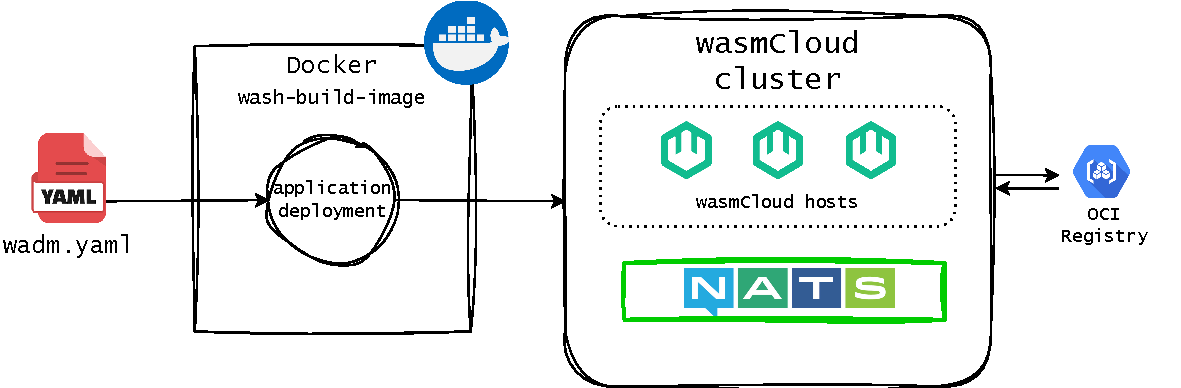
\includegraphics[width=0.8\textwidth]{img/schemi/schemi-architettura-deploy.drawio.pdf}
    \caption{Deployment applicazione Wasm su wasmCloud}
    \label{fig:code_deploy_pipeline}
\end{figure}
\FloatBarrier


\section{Networking fra componenti Wasm}

Il modello FaaS implementato in questo progetto necessita di appoggiarsi ad un sistema esterno per quanto riguarda lo scambio di informazioni fra componenti Wasm. In particolare è necessario utilizzare un sistema di messaggistica Pub/Sub distribuito in modo da disaccoppiare infrastruttura e parte applicativa e supportare l'esecuzione di funzioni quando viene ricevuto un evento (un messaggio in un topic).\\
La soluzione implementata è la stessa che wasmCloud utilizza per la comunicazione interna, cioè NATS. L'interfacciamento fra NATS e i componenti Wasm avviene tramite il provider messo a disposizione dal team di wasmCloud\footnote{\url{https://github.com/wasmCloud/wasmCloud/tree/main/crates/provider-messaging-nats}}.\\
La scelta di adottare NATS deriva da due motivi principali:
\begin{itemize}
    \item il sistema dovrebbe essere installato in ogni caso dato che server a wasmCloud per il routing dei messaggi
    \item la sua leggerezza e il supporto per l'ambiente Edge tramite i nodi Leaf lo rendono una soluzione ottima per gestire le necessità di questo progetto
\end{itemize}


\section{Considerazioni sulla soluzione}

La pipeline del framework è suddivisa nelle tre operazioni di generazione, build e deployment in modo che ognuna possa funzionare in modo autonomo (ovviamente se presenti i file necessari all'operazione).\\
Inoltre l'utilizzo di un container per le operazioni di build e deployment mira ad aumentare la compatibilità e la distribuzione del framework in modo che non sia dipendente dal sistema in cui verrà implementato: in questo progetto è stato fatto come CLI utilizzando Python, ma potrebbe essere anche esteso ad una configurazione SaaS completamente in Cloud o con approccio GitOps tramite actions e frameworks di CI/CD. 

